\part{Model Analysis}
 
\chapter{Burgers Equation}
\small
%\begin{quote}
%I feel sure that you do not understand how I came by
%my lonely ways. (Einstein about the statistical
%interpretation of quantum mechanics)
%\end{quote}
\begin{quote}
Some physicists. among them myself, cannot believe that we must abandon,
actually and forever, the idea of direct representation of physical reality
in space and time; or that we must accept then the view that events in nature
are analogous to a game of chance. (Einstein 1954)
\end{quote}

%\begin{quote}If God has made the world a perfect mechanism, He has at
%least conceded so much to our imperfect intellects that in order to
%predict little parts of it, we need not solve inumerable differential
%equations, but can use dice with fair success. (Born, on Quantum Physics)
%\end{quote}

\normalsize

\section{A Model of the Euler Equations}

As an instructive model of the 
Euler equations exhibiting basic aspects of
\emph{shock waves} and \emph{rarefaction waves}, 
we consider the following \emph{scalar conservation law}, referred to
as \emph{Burgers equation}:
Find the scalar function $u=u(x,t)$ such that
\begin{equation}\label{burgers}
\begin{array}{rcl}
\dot u +(f(u))^\prime &=&  0\quad\mbox{in }Q, \\
u(\cdot ,0)  &=&  u^0,
\end{array}
\end{equation}
where $f(u)=u^2/2$, $Q\equiv \bbR\times I$ with $I=(0,T]$,  
and we assume that the initial data 
$u^0(x)$ vanishes for large $\vert x\vert$.
%(which implies that $u(t,x)$ does the same for $t\in I$).
 
Burgers equation takes the pointwise form 
$\dot u+uu^\prime=0$ for a differentiable  pointwise solution $u$, which  
expresses that $u(x,t)$ is constant with values $u^0(\bar x)$
along straight lines $x=st+\bar x$ with slope $s=u^0(\bar x))$,
that is, along \emph{characteristics} defined by $\frac{dx}{dt}=u(x,t)$
with $x(0)=\bar x$. 

If $u^0(x)$ is increasing with increasing $x$ and is smooth, 
then there is a pointwise solution $u(t,x)$ for all time given by
the simple recipe 
\begin{equation}\label{uxu0}
u(x,t)=u^0(\bar x)\quad\mbox{for }
x=u^0(\bar x)t+\bar x.
\end{equation}
However, if the initial data $u^0(x)$ somewhere is
strictly decreasing, which of course will always be the case if 
$u^0(x)$ vanishes for large $\vert x\vert$, then characteristics will 
cross in finite time with different values and the solution 
formula gives conflicting function values, which can be 
interpreted as \emph{breakdown} of the pointwise solution. 
The result is 
that there is no differentiable function $u(x,t)$ satisfying
Burger's equation $\dot u+uu^\prime =0$ pointwise. 
We shall see
that this corresponds to the occurence of \emph{shocks}, 
which are represented by \emph{discontinuous} functions,
which satisfy the differential equation in a weak sense,
and in a pointwise sense only away from discontinuities
or jumps. 


What to do with an equation without pointwise solution? 
Of course, we regularize and consider instead the 
\emph{viscous/regularized Burgers equation}:
\begin{equation}\label{burgersreg}
\begin{array}{rcl}
\dot u +uu^\prime  -\nu u^{\prime\prime}&=&  0\quad \mbox{in }Q,\\
u(\cdot ,0)  &=&  u^0,
\end{array}
\end{equation} 
with $\nu >0$ a small viscosity. This problem can be solved
uniquely in a pointwise sense for all initial data, 
and as above the solution can be viewed as an approximate weak
solution to the original inviscid Burgers equation satisfying a 2nd
Law of the form
\begin{equation}\label{2ndlawBurgers}
\dot K(u;t)=-D_\nu (u;t)\quad\mbox{for }t\in I,
\end{equation}
where
\begin{equation}\label{KD}
\quad K(u;t)=\int_\bbR \frac{u(x,t)^2}{2}\, dx,\quad
D_\nu (u;t)=\int_\bbR\nu (u^\prime (x,t))^2\, dx.
\end{equation} 
The 2nd Law follows by multiplication of the viscous
Burgers' equation by $u$ and integration (by parts) with respect to $x$.


To give a perspective we now briefly recall the  
basics of the mathematical theory for conservation laws developed
in the 1950s motivated by the Euler equations of compressible
flow, in the model setting of Burgers equation. The basic idea is
to introduce the concept of \emph{weak solution} allowing discontinuous
solutions, and complement by a 2nd Law.  We shall see that the 2nd Law
singles out \emph{physical shocks}, which are discontinuous
weak solutions satisfying the 2nd Law, from \emph{non-physical shocks}
which are discontinuous weak solutions violating the 2nd Law.

We also present an alternative approach 
to single out physical shocks based on a stability analysis showing that a
a physical shock is stable and represents a
an observable physical phenomenon 
(like the ``bang'' from a supersonic airplane), 
while a non-physical shock is unstable and thus does not represent
any observable physical phenomenon.


%Before presenting the mathematicians solution we recall the basics:
%We thus a simple equation $\dot u+uu^\prime =0$ 
%which in general 
%\emph{has no pointwise solution}
%because of the inevitable occurence of shocks as soon as the initial
%data is decreasing. Similarly, the Euler equations 
%have no pointwise 
%solutions (except trivial solutions with constant velocity) because
%of the necessary appearnce of turbulence/shocks.

Burgers equation is formally reversible: If $u(x,t)$ is a 
pointwise solution in forward time on $[0,T]$, 
so is $-u(x,T-t)$ in reverse time. Burgers equation 
thus is formally reversible system, but in reality is irreversible, 
as a consequence of the non-existence of stable pointwise solutions. 
We thus use Burgers equation to illustrate that a World governed 
by the formally reversible Euler equations, is an irreversible
World, that is a world with an Arrow of time.




\section{Weak Solutions} 

A possibly
discontinuous function $u(x,t)$ is said to be a \emph{weak
solution to Burgers' 
equation} if 
\begin{equation}\label{burgersweak}\int_{\bbR\times\bbR_+} (-u\dot\varphi -f(u)\varphi^\prime )dx\, dt-
\int_\bbR u^0(x)\varphi (x,0)\, dx =0
\end{equation}
for all differentiable test functions $\varphi$ such that
$\varphi (x,t)$ vanishes for large $(x,t)$, assuming here
$I=(0,\infty )$.
%in $H^1(Q)$, where $Q=\bbR\times [0,T)$. 
This equation is obtained from (\ref{burgers}) by multiplication by
$\phi$ and integration by parts, shifting the derivatives
onto $\varphi$, thus allowing $u$ to be discontinuous. 

%A shock solution is thus 
%a weak solution but not a pointwise (strong) solution, since
%the differential equation is not defined at the point of the shock
%discontinuity. 



\section{The Rankine-Huginiot Condition}

A discontinuous function $u(x,t)$ defined by $u(x,t)=u_+$ if $x>st$ and 
$u(x,t)=u_-$ if $x<st$, where  $u_+$ and $u_-$ are two constant
states and $s$ is a constant, corresponding to a discontinuity 
propagating with speed $s$, is a weak solution
to Burgers' equation if the shock speed satisfies the 
\emph{Rankine-Hugoniot condition}
\begin{equation}\label{rh}
s=\frac{[f(u)]}{[u]},
\end{equation}
where $[u]=u_+-u_-$ and $[f(u)]=f(u_+ )-f(u_- )$. With $f(u)=u^2/2$
as in Burgers' equation, we have 
\begin{equation}\label{rhburgers}
s=(u_++u_-)/2.
\end{equation}
The Rankine-Hugoniot condition expresses the conservation law
(Burgers' equation)
in weak form for a piecewise constant discontinuous solution candidate $u$.


\section{Rarefaction wave}

The solution to Burgers equation with the \emph{increasing} 
discontinuous initial data $u^0(x)=0$ for $x<0$, and $u^0(x)=1$ for
$x>0$, is a \emph{rarefaction wave}
given by  
\begin{equation}\label{rarefaction}
\begin{array}{rcl}
u(x,t)&=& 0 \quad\mbox{for}\quad x<0,\\
u(x,t)&=& \frac{x}{t} \quad\mbox{for}\quad 0\le \frac{x}{t}\le 1,\\ 
u(x,t)&=& 1\quad\mbox{for}\quad 1< \frac{x}{t}.
\end{array}
\end{equation}
This is a continuous function for $t>0$
which satisfies (\ref{burgers}) pointwise
for $t>0$  off the lines $x=0$ and $x=t$ and can be viewed as
a pointwise solution (since it is continuous and piecewise
differentiable).
In a rarefaction wave, an
initial discontinuity separating two constant states develops into a 
continuous linear transition 
from one state to the other of width $t$ in space, 
corresponding to ``fan-like'' level curves in space-time as shown in
Fig. \ref{rarefactionfig}.
\begin{figure}[bhpt]
\begin{center}
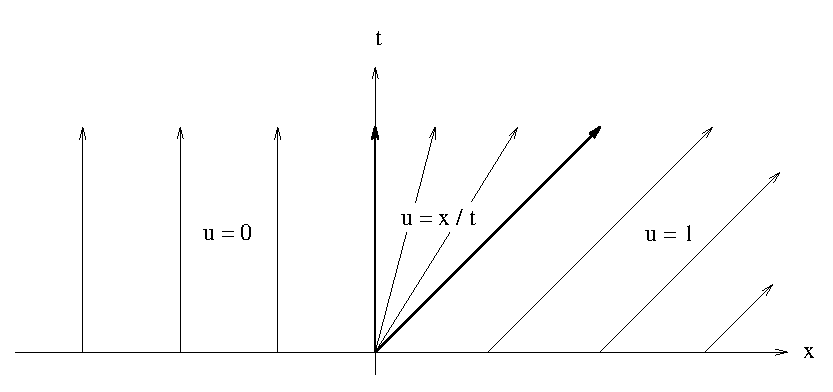
\includegraphics[height=3.3cm]{ambsthermopict/figRAchars.eps}
\caption{Characteristics of a rarefaction wave.}
\label{rarefactionfig}
\end{center}
\end{figure}
%\begin{figure}[bhpt]
%\begin{center}
%
\includegraphics[height=3.3cm]{figSHchars.eps}
%\caption{Characteristics of a shock}
%\label{shock}
%\end{center}
%\end{figure}






\section{Shock}

The solution with decreasing discontinuous initial data 
$u^0(x)=1$ for $x<0$, and $u^0(x)=0$ for
$x>0$, is a discontinuous \emph{shock wave} moving with speed $\frac{1}{2}$:
\begin{equation}\label{shock}
\begin{array}{rcl}
u(x,t)&=& 1 \quad\mbox{for}\quad x<\frac{t}{2},\\
u(x,t)&=& 0 \quad\mbox{for}\quad x>\frac{t}{2},  
\end{array}
\end{equation}
as shown in Fig \ref{shockfig}. We shall motivate that this is a 
\emph{physical shock}
satifying a 2nd Law.
\begin{figure}[bhpt]
\begin{center}
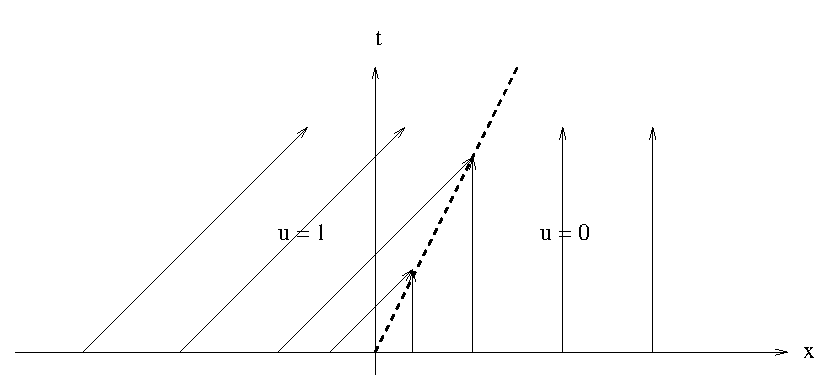
\includegraphics[height=3.3cm]{ambsthermopict/figSHchars.eps}
\caption{Characteristics of a shock}
\label{shockfig}
\end{center}
\end{figure}



\section{Weak solutions may be non-unique}

The rarefaction wave initial data 
$u^0(x)=0$ for $x<0$ and $u^0(x)=1$ for $x>0$, also admits
the alternative discontinuous weak solution 
\begin{equation}\label{unphyssol}
\begin{array}{rcl}
u(x,t)&=& 0 \quad\mbox{for}\quad x<\frac{t}{2},\\
u(x,t)&=& 1 \quad\mbox{for}\quad x>\frac{t}{2}, 
\end{array}
\end{equation}
corresponding to a discontinuity $\{x,t):x=st\}$ moving with speed
$s=\frac{1}{2}$. This solution is obviously
different from the rarefaction wave solution
(\ref{rarefaction}), which since it is a pointwise solution, also 
is a weak solution. Thus, we have in this case two different weak solutions, 
and thus we have an example of \emph{non-uniqueness of weak solutions.}
We shall see that the discontinuos solution (\ref{unphyssol}) 
violates the 2nd Law and thus is a \emph{non-physical shock solution}.
The physical solution in this case is the rarefaction wave
(which satisfies the 2nd Law with equality).



\section{The 2nd Law for Burgers Equation}

%The entropy inequalities are related to the Second Law of Thermodynamics
%stating that in a closed physical system, the entropy cannot
%decrease. Intuitively, the physical concept of ``entropy'' is related
%to ``disorder'' or ``loss of information'' and thus the  
%The Second Law states that disorder cannot decrease.
%To see how the Second Law in this form applies to the shock wave case above, 
%we note that the characteristics in this case ``converge into'' 
%the shock, which may be viewed as a ``loss of information'', or increase of entropy, 
%which is physically admissible.  On the other hand, for
%the unphysical solution (\ref{unphyssol}), the characteristics
%seem to ``emerge from'' the discontinuity, which may be viewed as
%some kind of ``creation of information'', which 
%would contradict the Second Law.
%Thus, in brief we may say that a discontinuous weak solution with
%the characteristics converging into the discontinuity, is a physical solution
%while it is unphysical if the characteristics are 
%divering out from the discontinuity.

We now check if (\ref{unphyssol}) satisfies the appropriate 
form of the 2nd Law (\ref{2ndlawBurgers})  
restricting space to $-1\le x\le 1$ and time to $0\le t\le 1$ assuming
the boundary conditions $u(-1,t)=0$ and $u(1,t)=1$. In this setting,
we obtain by multiplication of the viscous Burgers equation with $u$
and integrating by parts and using the sign of the viscous
term, the following form of the 2nd Law
\begin{equation}\label{2ndlawBurgers1}
-D_\nu (u;t)=  \dot K(u;t)+\int_{-1}^1(\frac{u^3}{3})^\prime =\dot K(u;t)+\frac{1}{3}
\end{equation} 
But for (\ref{unphyssol}) we have 
$\dot K=-\frac{1}{2}\frac{d}{dt}\frac{t}{2}=-\frac{1}{4}$, which
violates (\ref{2ndlawBurgers1}). 

Changing to the boundary conditions to $u(-1,t)=1$ and $u(1,t)=0$,
the 2nd Law changes to 
\begin{equation}\label{2ndlawBurgers2}
-D_\nu (u;t)= \dot K(u;t)+\int_{-1}^1(\frac{u^3}{3})^\prime =\dot K(u,t)-\frac{1}{3},
\end{equation} 
which is satisfied by (\ref{shock}) since now
$\dot K=\frac{1}{2}\frac{d}{dt}\frac{t}{2}=\frac{1}{4}<\frac{1}{3}$.

We conclude that a  discontinuous function $u(x,t)$ with the constant
states $u_-$ for $x<st$ and $u_+$ for $x>st$ corresponds
to a physical shock solution with shock speed $(u_-+u_+)/2$
if $u_-> u_+$, and to a non-physical 
shock if $u_-<u_+$.

We furher see that a shock dissipates substantial
kinetic energy into heat since for a viscous profile of width
$\nu$ joining two states $u_-$ and $u_+$   
\begin{equation}\label{Djump}
D_\nu (u;t)\equiv \int_\bbR\nu (u^\prime )^2\, dx\approx (u_--u_+)^2
\end{equation}
for small $\nu$.


\section{Burning Books}

The 2nd Law states that the characteristics of 
a physical shock  ``converge into'' the shock, corresponding
to $u_->u_+$. For the unphysical shock solutin
corresponding to the rarefaction
initial data with $u_-<u_+$, the characteristics
appear to ``emerge from'' the discontinuity. The
2nd Law thus allows information (features of the solution) to 
be ``destroyed'' (in a shock with converging characteristics), 
but not ``created out of nothing'' 
(in an unphysical rarefaction with diverging characteristics).
This connects to the essence of irreversibility: Burning books
can readily be done without any sophistication, while recovering the
original text from the ashes is impossible.  

\section{Stability of a Rarefaction Wave}

We shall now see that the 2nd Law can be replaced by a stability analysis
in its main mission to distingush physical shocks from unphysical shocks.
This reflects the fact that a stable process can be physically realized 
and observed, while an unstable process will have no permanence and
thus will be very difficult (or impossible) to realize.

The stability of a solution $u(x,t)$ is governed 
by the linearized equation 
\begin{equation}\label{linburgers}
\dot w+(uw)^\prime =0\quad\mbox{in }\bbR\times\bbR_+
\end{equation}
where $w$ represents a (small) perturbation (tending to zero for $\vert x\vert$
tending to infinity), and the solution $u$ acts as a 
given coefficient. The growth properties of the solution
$w$ of the linearized equation determines the stability:
If $w$ grows quickly in time, then the solution $u$ is unstable,
and if $w$ stays bounded, then $u$ is stable. Of course, stability
connects to finite precision: the level of the perturbation 
represents the precision.

We first consider the case of
a rarefaction wave given by (\ref{rarefaction}). Multiplying by $w$ and
integrating in space, we obtain by a simple computation using the fact
that $u^\prime (x,t)=1/t$ for $0\le x\le t$ and $u^\prime (x,t)=0$ else,
\[
\frac{d}{dt}\int_\bbR w^2(x,t)\, dx+
\int_0^t w^2(x,t)\frac{1}{t}\, dx =0,\quad\mbox{for }t>0,
\]
from which follows that
\begin{equation}\label{stabrarefaction}
\int_\bbR w^2(x,t)\, dx\le \int_\bbR w^2(x,0)\, dx\quad\mbox{for }t>0.
\end{equation}
This inequality shows that the $L_2$-norm in space
of a perturbation from initial data does not grow with time, 
which proves stability 
of a rarefaction wave. Note that this
argument builds on the fact that the rarefaction wave $u(x,t)$ is increasing in $x$ so that $u^\prime$ is
non-negative.

\section{Stability of Shock}

The stability proof used above to prove stability of a rarefaction
wave, does not work the same way for a shock, since in this case
$u(x,t)$ is decreasing with $x$. In fact a shock does not satisfy an
$L_2$ stability estimate of the form (\ref{stabrarefaction}). However,
one can prove instead an $L_1$-bound of the form
\begin{equation}\label{stabshock}
\int_\bbR \vert w(x,t)\vert\, dx\le \int_\bbR \vert w(x,0)\vert
\, dx\quad\mbox{for }t>0.
\end{equation}
This follows by multiplying (\ref{linburgers}) by $sgn (w)=+1$ if $w>0$ 
and $-1$ if $w<0$, to get by integration by parts:
\begin{equation}\label{linburgersL1}
\frac{d}{dt}
\int_\bbR\vert w(x,t)\vert\, dx +(u_--u_+)\vert w(\frac{t}{2},t)\vert =0,
\end{equation}
and using the fact that for a shock $u_+<u_-$.
Moreover, we will below with a different type of stability estimate
show that a shock is stable from computational RNS point of view, 
Thus, a shock is a stable phenomenon from both physical and computational
point of view.

%In one space dimension, shocks exist as piecewise constant
%(discontinuous) solutions, while in three space dimensions
%shocks in general generate turbulence. We present evidence in Vol 5.   

\section{Instability of Non-Physical Shock}

We saw above that the rarefaction wave solution is stable, and we now
study the stability of the alternative weak solution (\ref{unphyssol}).
By the same argument as used to prove (\ref{linburgersL1}) we obtain
\begin{equation}\label{linburgersL1unstable}
\frac{d}{dt}\int_\bbR\vert w(x,t)\vert\, dx =(u_+-u_-)\vert w(\frac{t}{2},t)\vert , 
\end{equation}
where now $u_+>u_-$. In this case, $\int_\bbR\vert w(x,t)\vert\, dx$
can grow arbitrarily fast, since the positive right hand side
in (\ref{linburgersL1unstable}) in no way can
be controled by the left hand side. We thus conclude that an 
unphysical shock is unstable.

\section{2nd Law $=$ Stability $+$ Finite Precision}
We thus have two methods
to single out physical shocks, one based on stability,
and the other based on the 2nd Law. This shows that ultimately the 2nd Law
expresses a stability condition, reflecting that Nature only can realize
phenomena which are properly stable, in its analog finite precision
computation. We thus may view the 2nd Law to express 
a combination of stability and finite precision.   


\section{A Traffic Model}

The equation (\ref{burgers}) with $f(u)=u(1-u)$ models the flow 
of cars along a highway represented by the $x$-axis with
$0\le u\le 1$ the car density and $0\le v=(1-u)\le 1$ the 
car velocity as a function of density: Sparse cars ($u\approx 0$)
move fast ($v\approx 1$) and packed cars ($u=1$) stand still
($v=0$). The equation (\ref{burgers}) then expresses
conservation of mass in the sense that there are no side roads
through which cars can enter or exit (and they cannot simply disappear
into the sky). 

We understand that if $u(x,t)$ is increasing
in $x$ so that the car density increases in the direction of motion,
then the car velocity will be decreasing in the direction of motion
which means that 
faster cars behind will approach slower cars ahead.
 But the $x$-axis
is a one-lane street and does not allow a faster car to overtake a slower
car, and so 
eventually faster cars will have to break in order to not run 
into slower cars ahead, that is, the law $v=(1-u)$ will have to
be violated and thus the conservation law (\ref{burgers})
cannot be satisfied pointwise. In the inviscid equation (\ref{burgers})
this will correspond to the appearence of a shock. The corresponding
regularized equation takes the form
\[
\dot u +((u(1-u))^\prime -\nu u^{\prime\prime} =0,
\]
which we formally can write as
\[
\dot u +(uv)^\prime =0
\]
with the modified velocity law
\[
v=(1-u-\frac{\nu}{u} u^\prime ),
\]
with the effect that in the dangerous case of 
increasing density ($u^\prime >0$),
faster cars will be slowed down more than slower cars and
collisions from behind will thus be avoided.

In this model the shock corresponds to the well-known situation 
when an inexperienced driver suddenly steps on the brake to avoid
collision into a cue, which in the regularized problem 
corresponds to the smoother action of an experienced driver
slowing down because the car density is larger
ahead than behind.





\section{Non-Existence Exact Euler Solutions}

We have seen that the inviscid Burgers equation has discontinuous
shock solutions, which can be viewed as weak solutions satisfying
a 2nd Law. One can thus speak about a shock solution as an exact 
weak solution of Burgers equation satisfying a 2nd Law, and 
this solution is the limit of regularized solutions as the 
viscosity tends to zero.
The goal of the classical mathematical analysis of conservation laws
based on regularization, is to establish a corresponding result for
the Euler equations: The goal is thus to prove the existence of a function
satisfying the Euler equations in a weak sense together with a 2nd Law,
as a limit of regularized solutions.

However, this goal has not been reached, and we have good reasons
to believe that it cannot be reached. This is 
because of the appearence of turbulent solutions to the 
regularized Euler equations which do not seem have a limit in the form
of a function. It is thus not meaningful to speak about 
exact solutions to the Euler equations, because such objects do not
exist, but we may speak about regularized solutions because
they do exist and we may view such solutions as approximate
solutions to the Euler equations.

With this perspective it is reasonable to view a shock solution
not as is usual as an exact weak solution to the Euler equations, 
but rather to view a viscous shock solution, an exact solution to the 
regularized Euler equations, as an approximate solution to the 
Euler equations. 
Thus only strong pointwise solutions could deserve the
title of ``exact solution''; a weak solution 
which is not a strong solution like a shock, could only be an approximate 
solution. This may seem to differ from the common way of looking at 
weak solutions of differential equations, as functions satisfying
the differential equation ``weakly exactly'', but this is not completely
natural since the notion of ``weakly'' has an element of ``inexactly''
built in. Only a strong pointwise solution can be an exact solution.
I somebody offers you to buy an unknown painting by
van Gogh,  which you are only allowed to inspect from a distance
of 10 meters, you may get suspicious and refrain from a deal.

 

\chapter{BurgersRNS}

\small
\begin{quote} But maybe that is our mistake: 
maybe there are no particle positions and velocities, but only waves. 
It is just that we try to fit the waves to our preconceived ideas of 
positions and velocities. The resulting mismatch is the cause of the 
apparent unpredictability. (Stephen Hawking 1988)
\end{quote}
\normalsize  

\section{Introduction}
We will now consider RNS applied to Burgers' equation as a simple
version of RNS. We recall that RNS is Galerkin's 
finite element method
combined with a weighted least-squares control of the
residual. RNS is based on  piecewise polynomial approximation
in space-time and offers spectrum of computational methods 
depending on the choice of the space-time
mesh, as presented in detail in \cite{cde,ambsflow}.
RNS uses piecewise polynomials which are
continuous in space and possibly discontinuous in time.
These variants are referred to as cG($p$)cG($q$) or cG($p$)dG($q$) with
cG($p$) referring to continuous piecewise approximation of degree $p$
in space, and cG($q$)/dG($q$) referring to  continuous/discontinuous
approxiamtion in time of degree $q$. RNS is \emph{Eulerian} if
the space-time mesh oriented along the space and time coordinate axis, 
is \emph{Lagrangean} if the space-time mesh is oriented along particle
paths in space-time, and \emph{Arbitrary Lagrangean-Eulerian} or \emph{ALE} 
if the space-time mesh is oriented according to some other feature such as
space-time gradients of the solution. 
Lagrangean variants are also referred to as \emph{characteristic Galerkin}, 
and Eulerian variants as \emph{streamline diffusion methods}.

In all these variants the space-time mesh is usually organized in
space-time slabs between discrete time levels, and RNS then
gives a time-stepping method allowing the solution to be
computed form one time level to the next progessing in time. The
space mesh may be changed across the discrete time levels to avoid 
mesh distortion and allow mesh adaption. In dG($q$) the
approximation is discontinuous in time and the space
mesh may vary from one slab to the next. If the space mesh is changed 
across a discrete time level in cG(q), then
a projection from the previous mesh 
to the new mesh is performed. The projection is built 
into the Galerkin method  through a jump term corresponding to a 
$L_2$ projection. The discrete solution between the
discrete time levels may be viewed as an approximate {\em transport} step,
and the whole process may be viewed as a method of the basic form
\emph{projection-transport}. 

The traditional finite difference methods are of Eulerian type with the 
first order Lax-Friedrichs' scheme from the 50s as a prototype on 
conservation form  
and with artificial viscosity proportional to the mesh size. The next 
generation
of classical schemes originates from Godunov's method in 1d, 
which is of the form projection-transport with piecewise constant 
(discontinuous) approximation  and a Riemann solver for the transport step. 
The multi-dimensional finite volume schemes 
developed in recent decades, use discontinuous polynomial
approximation with numerical fluxes often constructed using
1d Riemann solvers. 
All these methods may alternatively be viewed as particular 
RNS methods. 


%Galerkin/least squares methods were pionereed in the early
%1980s by Hughes followed by Johnson in the form of 
%streamline diffusion methods, see \cite{hughes}, \cite{johnson}, \cite{cime}.
 
\section{Semi-Discrete RNS for Burgers Equation}

For the purpose of analysis displaying essential aspects,
we consider a \emph{semi-discrete} RNS method for Burgers equation with
cG(1) discretization in space. Full discretization
with cG(q) or dG(q) in time can be analyzed similarly.
Let then for a
given mesh on $\bbR$ with 
mesh size $h$, $V_h$ be the set of continuous functions $v(x,t)$ 
which for $t\in I=[0,T]$ are piecewise linear in $x$ on the mesh.
The simplest version of semidiscrete RNS takes the form: 
Find $U\in V_h$ such that
\begin{equation}\label{RNSburgers} 
  ((R(U),v))+((hU^\prime ,v^\prime ))=0\quad\forall v\in V_h,
%+(\hat\epsilon \nabla U,\nabla v)_n
%  +([U_{n-1}],v_{n-1}^+)_\bbR =0,\quad\forall v\in V _n,
\end{equation}
where $R(U)=\dot U+UU^\prime$ is the Burgers residual, $((v,w))=\int_Q vw\, dxdt$ with $Q=\bbR\times I$ and $U(x,0)\in V_h$ 
interpolates $u^0(x)$. 
This is equivalent to a  system of ordinary differential equations
in time. We have here replaced residual stabilization by
$(hU^\prime ,v^\prime )$, and we thus consider 
a Galerkin method in space for a viscous Burgers equation
with viscosity $\nu =h$.    

%\[
%\delta =\frac{1}{2}(k_n^{-2}+h_n^{-2}A(U)^2)^{-1/2},
%\] 
%$\hat\epsilon =\max (\epsilon ,\gamma_1h^{2-\kappa}R(U),\gamma_2h^{\frac{3}{2}})$, and
%now $R(U)=\vert \dot U+A(U)U^\prime \vert + \vert [U_{n-1}]\vert/k_n$ on $S_n$. 
\section{Basic Energy Estimate as 2nd Law}

Choosing $v=U$ in (\ref{RNSburgers}), we obtain by 
integration by parts over $\bbR$ the following direct analog
of (\ref{2ndlawBurgers}):
\[
\dot K(U;t)=-D_h(U;t),\quad\mbox{for } t\in I.
\]
%
%\[
%K(U;t)=\frac{1}{2}\int_{\bbR} U^2(t)dt,
%\quad D_h(U;t)=\int_0^t\int_\bbR h(U^\prime )^2\, dxdt.
%\]
%This is the basic energy estimate for RNS for Burgers'equation,
%which is also a 2nd Law for the kinetic energy $K$.
In the presence of shocks, $D_h(U; t)$ will be substantial
and thus $U'$ will at shocks be large ($\sim h^{-1})$.



%\section{RNS and the 2nd Law}

%We shall now prove as a major observation of this note that
%RNS automatically satisfies the entropy inequality (\ref{entropyineq})
%in a weak sense, and thus automatically computes a physical solution
%without explicitely enforcing the entropy inequality. The key point is
%thus that construction of RNS as weak satisfaction of the conservation
%law combined with weighted least squares constrol of the pointwise
%residual, assures that a RNS solution also satisfies the entropy
%inequality characterizing physical solutions. In particular, there
%is no chance that RNS will produce an non-physical solution
%violating the entropy condition.

%To see this, we choose a smooth non-negative
%test function $\varphi$, write $w=\varphi  U$ and then choose
%in RNS the finite element test function $v=w_h$, where
%$w_h\in V_h$ is a nodal interpolant of $w$, noting that $w$ does
%not belong to $V_h$ in RNS in general. We then have with
%$\tilde U_n=\frac{1}{2}(U_n^++U_n^-)$, by integration by parts in space and time,
%\[ 
% -(\frac{1}{2}U^2,\dot\varphi )_{Q_N}
%-(\frac{1}{3}U^3,\varphi^\prime )_{Q_N}
%\]
%\[
%=\sum_{n=1}^N\bigl((R(U),w)_{S_n} +([U_{n-1}],
%\tilde U_{n-1}\varphi_{n-1}^+)_\bbR\bigr) 
%\]
%\[
%=\sum_{n=1}^N\bigl(R(U),\hat w_h)_{S_n}-(hR(U),\dot w_h+
%Uw_h^\prime )_{S_n}
%  +([U_{n-1}],\tilde U_{n-1}\varphi_{n-1}^+- w_{h,n-1}^+)_\bbR\bigr)
%\]
%\[
%\equiv I+II+III,
%\]
%where $\hat w_h=w-w_h$, and we used (\ref{RNSburgers}) with $v=w_h$.
%We now estimate the interpolation error $\hat w_h$ as follows:
%\[
%\Vert \hat w_h\Vert_{S_n}\le \Vert h^2D^2w\Vert_{S_n}\le Ch\Vert U\Vert_\infty ,
%\]
%where $D$ represents first order derivation in space or time,
%$C$ depends on first and second derivatives of $\varphi$
%and $\Vert U\Vert_\infty =\max_{Q_N}\vert U\vert\equiv M$. This type of estimate is 
%referred to as super-approximation since it contains the factor $h$ without paying the price 
%of first derivatives of $U$, which results from the special form of $w=\varphi U$ as a product
%of a finite element function $U$ and a smooth function. We conclude that
%\[
%I\le  CM\Vert hR(U)\Vert_{Q_N}\le CM\sqrt{h},
%\]
%where we used the basic energy estimate assuming $\Vert u^0\Vert\sim 1$. Further
%\[
%II=\sum_{n=1}^N(hR(U),\frac{\partial}{\partial t} \hat w_h+
%U\hat w_h^\prime )_{S_n}-\sum_{n=1}^N(hR(U),\dot w+
%Uw^\prime )_{S_n}=II_a+II_b.
%\]
%We have again by super-approximation and the energy estimate that
%$II_a\le CM\sqrt{h}$, and 
%\[
%II_b = -\sum_{n=1}^N(hR(U),\dot U\varphi +
%UU^\prime\varphi )_{S_n}-\sum_{n=1}^N(hR(U),U\dot\varphi +
%UU\varphi^\prime )_{S_n}
%\]
%\[
%\le -\sum_{n=1}^N(hR(U),R(U)\varphi )_{S_n}+CM\sqrt{h}\le CM\sqrt{h},
%\]
%where we used the non-negativity of $\varphi$. The term $III$
%is estimated similarly. We conclude that for all non-negative
%test functions $\varphi$, we have
%\[ 
% -(\frac{1}{2}U^2,\dot\varphi )_{Q_N}
%-(\frac{1}{3}U^3,\varphi^\prime )_{Q_N}\le CM\sqrt{h},
%\] 
%where $M$ is a bound for $U$ and $C$ depends on up to second derivatives
%of $\varphi$. This expresses that the RNS solution $U$
%approximately satisfies the entropy inequality in weak form
%and the approximation improves as $h$ gets smaller. We refer to this property of RNS
%as entropy consistency. In particular
%RNS cannot compute a non-physical solution significantly
%violating the entropy inequality significantly. Note that the $M$-bound on $U$ is natural
%and can be proved by a maximum principle if RNS is suitably modified.  

%We have now established the key feature of RNS to automatically satisfy
%the entropy inequality approximately, as a consequence of the
%least squares stabilization. The key to the proof is the super-approximation
%making it effectively possible to choose $U\phi$ as a test function in RNS, 
%from which entropy consistency follows using the positivity of the least squares
%term, which reflects that
%the entropy inequality is obtained by multiplication of the viscid Burgers' equation
%by $\eta^\prime (u)\varphi =u\varphi$. Note that choosing $U$ as a test function 
%gives the basic energy estimate, which is the integrated form of the entropy
%inequality, and the step to choose instead $(U\phi )_h$ is not 
%large, but requires the least squares stabilization to work out





\section{A Posteriori Error Estimation by Duality}

We shall now prove we the following a posteriori 
error estimate, where $u$ is the solution of the viscous Burgers equation 
with $\nu =h$:
\begin{equation}\label{apostburgers}
\Vert u-U\Vert_{Q}\le S\Vert hR(U)\Vert_{Q},
\end{equation}
where $\Vert\cdot\Vert_Q$ is the $L_2(Q)$-norm and 
\begin{equation}\label{stabburgers}
S=\frac{\Vert h\phi^{\prime\prime}\Vert_{Q}
}{\Vert e\Vert_{Q}},
\end{equation}
is a stability factor defined by the solution 
$\varphi$ of the following 
linearized dual problem:
\begin{equation}\label{burgdual}
\begin{array}{rcl}
 -\dot\varphi - 
a\varphi^\prime -
h\varphi^{\prime\prime}  =  e, & & \mbox{in }Q,\\
\varphi (x,t)  \rightarrow  0, & & x\rightarrow \pm\infty ,t\in I , \\
\varphi (x,T)  =  0,  & & x\in \bbR ,
\end{array}
\end{equation}
{\flushleft where} $a=(u + U)/2$. We notice that the dual problem
has a viscous term with viscsoity coefficient $h$.



To prove the a posteriori error estimate (\ref{apostburgers})
we multiply (\ref{burgdual}) by $u-U$ and integrate in space and time
to get the error representation
\[
\Vert u-U\Vert_{Q}^2=((R(U),\phi ))+((hU^\prime ,\varphi^\prime )).
\]
We then use the Galerkin orthogonality (\ref{RNSburgers})
with $v=\Phi\in V_h$ an interpolant of the dual solution $\varphi$, to get
\[
\Vert u-U\Vert_{Q}^2=((R(U),\phi -\Phi ))+
((hU^\prime ,\varphi^\prime -\Phi^\prime )),
\]
which combined with an interpolation error bound of the form 
\[
\Vert\varphi -\Phi\Vert_{Q}+\Vert h(\varphi^\prime -\Phi^\prime )\Vert_{Q}\le
C_i\Vert h^2\varphi^{\prime\prime}\Vert_{Q},
\]
where $C_i$ is an interpolation constant, shows that
\[ 
\Vert u-U\Vert_{Q}^2\le C_i\Vert hR(U)\Vert_{Q}\Vert h\varphi^{\prime\prime}\Vert_{Q},
\]
where $R(U)$ has been augmented by the contribution $\Vert hU^\prime\Vert_Q$,
which proves (\ref{apostburgers}), setting $C_i=1$ for simplicity.

By the basic energy stability estimate, we have
\[
\Vert hU^\prime\Vert_{Q}\le\sqrt{h}\quad \mbox{if }\Vert u^0\Vert_\bbR =1,
\]
suggesting the same estimate for $\Vert hR(U)\Vert_Q$, 
which of course is checked a posteriori, and thus we expect
\begin{equation}\label{apostburgers2}
\Vert u-U\Vert_{Q}\le S\sqrt{h} .
\end{equation}
We shall now prove that for a shock $S\sim 1$, which shows that
a shock is computable with RNS, with a $L_2(Q)$ error of size $\sqrt{h}$, which
is optimal from approximation point of view (if we consider 
the exact solution $u$ to be discontinuous) 
and $U$ is continuous in $x$ on the mesh.


\section{Stability Estimate for a Shock}

We shall now investigate the stability properties of the dual problem
(\ref{burgdual}) and seek to bound 
$h\phi^{\prime\prime}$ in terms of the right hand side
$e$. For simplicity we linearize at the exact solution 
$u(x,t)$ (instead of the mean value
$(u+U)/2$) and thus consider the dual problem
\begin{equation}\label{burgdual1}
\begin{array}{rcl}
 -\dot\phi - 
u\phi^\prime -
h\phi^{\prime\prime}  =  e, & & \mbox{in } Q,\\
%\phi (x,t)  \rightarrow  0, & & x\rightarrow \pm\infty ,  \\
\phi (\cdot ,T)  =  0.
\end{array}
\end{equation}
The stability properties are largely determined by the sign of $u^\prime$,
which reflects the change of the direction $u$ of the characteristics. If
$u^\prime \le 0$, then the characteristics converge with increasing $t$,
which typically occurs in the case of a shock. If $u^\prime \ge 0$,
then the characteristics diverge, which typically occurs in the
case of a rarefaction. If $u^\prime $ is bounded below by a moderate
constant, e.g. $u^\prime\ge 0 $,  then we may
estimate $\Vert \phi\Vert_{L_\infty (L_2(\bbR ))}$ and
$\Vert\sqrt{h}\phi^\prime\Vert_Q$  in terms of a moderate constant
times $\Vert e\Vert_{Q}$, which we refer to as 
{\it weak stability}. 
If $u^\prime$ is bounded above by a moderate constant, 
e.g. $u^\prime\le 0$, 
then we may estimate $\Vert h\phi^{\prime\prime}\Vert_{Q}$ in terms of
a moderate constant times $\Vert e\Vert_{Q}$, which we refer to as {\it strong stability},
because we estimate second derivatives of $\phi$, cf. (\ref{stabburgers}). 
These estimates are proved by multiplying by $\phi$ and 
$-h\phi^{\prime\prime}$, respectively,
bringing in the positive stabilizing terms 
$\frac{1}{2}u^\prime \phi^2$ and $-\frac{1}{2}h u^\prime (\phi^\prime )^2$,
respectively.

We now give the details in the case of a shock with $u^\prime\le 0$, where
we assume $u$ is differentiable with a very large negative $x$-derivative
close to the shock.  We indicate the general nature of the characteristics of the dual problem 
in Fig \ref{chardualshock}.  
We shall prove that the solution $\phi$ of (\ref{burgdual1}) satisfies
\begin{equation}\label{strongstabest}
\Vert{h}\phi^{\prime\prime}\Vert_{Q}+
\Vert\dot\phi+u\phi^\prime\Vert_{Q}
+\sup_{0<t<T}\Vert{h}^{1/2}
\phi^\prime (\cdot , t)\Vert_{R}
\leq 3\Vert e\Vert_{Q}.
\end{equation}
To see this we multiply the first equation in (\ref{burgdual1}) by
$-h\phi^{\prime\prime}$, integrating by parts with respect to $x$, 
and integrating in time over $(\tau ,T)$ with $0<\tau <T$,
we get with $Q_{\tau} =\bbR\times (\tau ,T)$
\begin{equation}\begin{array}{l}
\frac{1}{2}\int_{\bbR}h\left(
\phi^\prime (\cdot ,\tau )\right)^2 dx 
+\int_{Q_{\tau}}\left(h\phi^{\prime\prime}\right)^2\,dxdt +\int_{Q_{\tau}}\frac{1}{2}
\left(uh\left(\phi^\prime\right)^2\right)^\prime ~dxdt  \vspace{4mm} \\
 \leq \frac{1}{2}\int_{Q_{\tau}}\left({h}u^\prime
\left(\phi^{\prime}\right)^2+e^2+\left(h\phi^{\prime\prime}\right)^2\right)~\mbox{d}x\mbox{d}t,
\end{array}
\end{equation}
which proves the desired result stating that $S\sim 1$ for a shock.

\begin{figure}[ht]\label{chardualshock}
\centerline{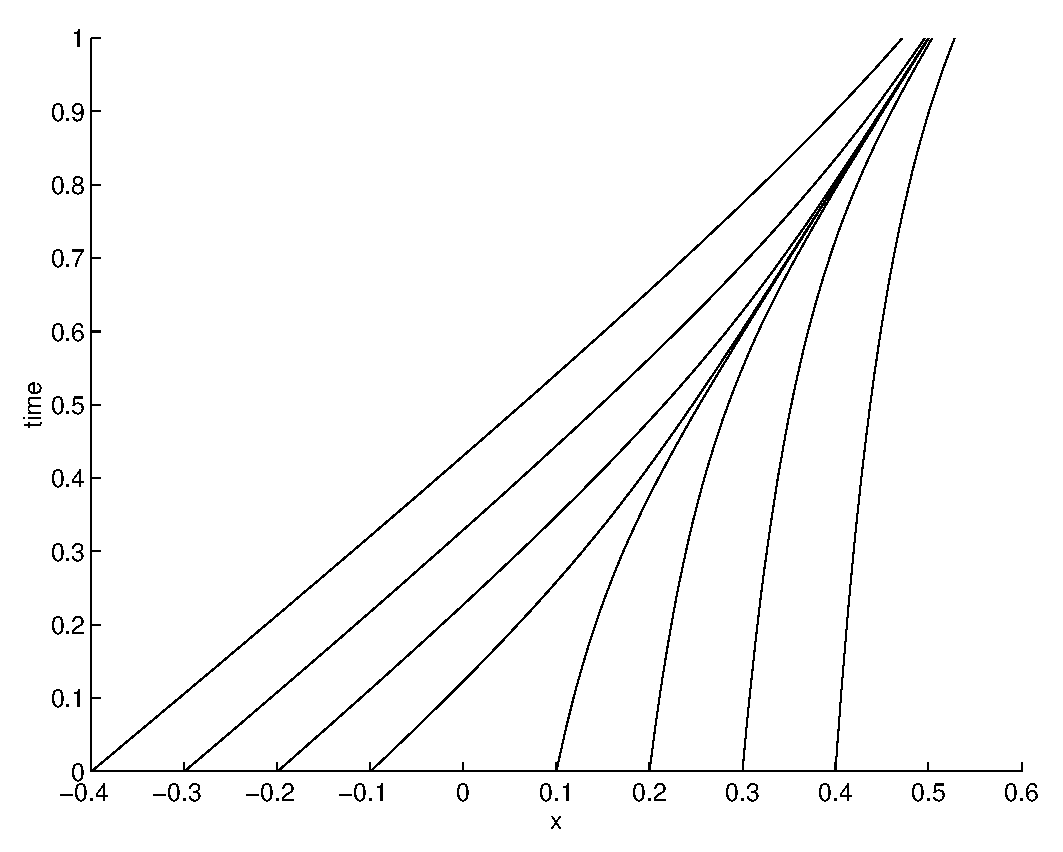
\psfig{figure=ambsthermopict/figCHARS.eps,height=2.5in,width=4in}}
\caption{Characteristics of the dual problem for a 
regularized shock solution.}
\end{figure}


As comparison, let us now attempt to derive a weak stability  estimate 
for (\ref{burgdual1}) in the case $u$ is a shock.
Multiplication 
by $\phi$ and integration over $Q_\tau$ gives
\[
\begin{array}{l}
 \frac{1}{2}\int_R
\phi^2(x,\tau )~dx + h\int_{Q_\tau}\left(
\phi^\prime (x,t)\right)^2~dxdt \vspace{3mm}\\
= -\frac{1}{2}\int_{Q_\tau}u^\prime 
\phi^2(x,t)~dx +\int_{R}e(x,t) \phi(x,t)~dx .
\end{array}\]
Since $u^\prime$ is large negative in the case of a shock, we have
large positive term of the right hand side, and using a Gronwall
inequality would results in a very large stability
factor. On the other hand, we show below weak stability for a 
rarefaction wave with $u^\prime\ge 0$, reflecting the 
above stability result for the perturbation equation.



Summing up, we see that for a shock, the linearized dual problem statisfies a strong
stability estimate with a stability factor of moderat size, while
a corresponding weak stability estimate appears to have a very large
stability factor. These stability features may be understood in a qualitative
sense, by pondering the directionality of the characteristics and the nature
of the $L_2$-norm. 

\section{Stability Estimates for a Rarefaction Wave}

We now consider the linearized dual Burgers' equation (\ref{burgdual1}),
linearized at the exact solution $u(x,t)=x/t$, corresponding to a rarefaction wave. 
Multiplying now (\ref{burgdual1}) by 
$-ht\phi^{\prime\prime}$, and using standard manipulations,
we obtain the following weighted norm strong stability estimate for $0<\tau <T$,
\begin{equation}\label{weightedstrongstab}
\Vert\tau^{1/2}h^{1/2}\phi^\prime\Vert 
+\Vert \omega h\phi^{\prime\prime}\Vert_{Q_\tau }
\leq \Vert \omega e\Vert_{Q_\tau } ,
\end{equation}
where $\omega (t)=t^{1/2}$ acts as a weight. 

A weighted norm analog of the a posteriori error estimate (\ref{apostburgers}) takes the form
\begin{equation}\label{weightedapostburger}
\Vert \omega^{-1} e\Vert_{Q_N}\le S_\omega\Vert \omega^{-1} hR(U)\Vert_{Q_N}
\end{equation}
with $S_\omega$ defined by the direct weighted norm analog of (\ref{stabburgers}).
The estimate (\ref{weightedstrongstab}) then shows that $S_\omega \sim 1$, 
and thus a rarefaction wave solution is computable in the weighted
norm with computational work corresponding to interpolation.
Note that the presence of the weight $t^{-1/2}$ will force more
stringent demands on the mesh for $t$ close to zero, which will
force an accurate resolution of the initial phase of the rarefaction.
This is intuitively reasonable and corresponds to the fact that an initial
error in the computation of a rarefaction will get amplified as time goes,
because characteristics diverge forward in time. On the other hand,
in the case of a shock, an initial error may be eliminated at later times,
because of converging characteristics, Thus, a rarefaction is more delicate
to compute than a shock, which we will see in the computational results 
we now present.





\section{Dual Solution and Stability Factors}

We display below RNS computations of a combination of  
a rarefaction wave and a shock using the cG(1)dG(0)-
method on a uniform space mesh with $h=10^{-3}$
and time step $10^{-4}$ taken from \cite{burman}.  We plot 
the computed solution at t=0,  t=0.3 , t=0.8, t=1 in Fig \ref{shockrarefaction}.
We see that the initial discontinuity
develops into a rarefaction and that a shock is formed for $t\approx 0.5$.

\begin{figure}[bhpt]
%\begin{center}

\includegraphics[height=4cm]{initburger}

\includegraphics[height=4cm]{03Tburger}

\includegraphics[height=4cm]{08Tburger}

\includegraphics[height=4cm]{Tburger}
\caption{A combined rarefaction and shock wave}
\label{shockrarefaction}
%\end{center}
\end{figure}


We solve the dual problem
using the following different approximations of the coefficient $a=(u+U)/2$
and the error $e$, with $\bar u$ the analytical, inviscid solution, 
and $U(h)$ the finite element solution on a mesh of size $h$:
(i) $a=(\bar u+U(h))$ and $e=\bar u-U(h)$,
(ii) $a=U(h)$ and $e=\bar u-U(h)$, (iii) $a=(U(h/4)+U(h))/2$ and $e=U(h/4)-U(h)$. 
We plot the corresponding dual solutions $\phi$ 
at the same time levels as above, but in revers
e order (t=1, t=0.8, t=0.3 , t=0)
in Fig \ref{dualsolution}.
\begin{figure}[bhpt]\label{dualsolution}
%\begin{center}

\includegraphics[height=4cm]{bdual10}

\includegraphics[height=4cm]{bdual08}

\includegraphics[height=4cm]{bdual03}

\includegraphics[height=4cm]{bdual00}
\caption{Dual solution in reverse time.}
%\end{center}
\end{figure}
We also plot in Fig. \ref{dualsol2} the corresponding second 
derivatives $\phi^{\prime\prime}$. 
\begin{figure}[bhpt]
%\begin{center}

\includegraphics[height=4cm]{bdualxx10}

\includegraphics[height=4cm]{bdualxx08}

\includegraphics[height=4cm]{bdualxx03}

\includegraphics[height=4cm]{bdualxx00}
\caption{Second deriatives of the dual solution in reverse time}
\label{dualsol2}
%\end{center}
\end{figure}
We note the change of $\vert\phi^{\prime\prime}\vert$, which may be viewed as a weight
in the a posteriori error estimate, from being 
large close to the shock at final time towards being large 
close to the initial discontinuity at $(x,t)=(0.2,0)$ initiating the rarefaction.
We see that that it is the data from the rarefaction at final time which
generates the large values of $\phi^{\prime\prime}$ at $t=0$, and not those
from the shock. This indicates that a rarefaction is more delicate to compute than a shock. 


We plot in Fig. \ref{stabfactorstrong} the strong stability factor $S$ defined
by (\ref{stabburgers})
for (i)-(iii) and $h=0.0001, \,h=0.00005, \,h=0.00001$.
\begin{figure}
%\begin{center}

\includegraphics[height=6cm]{S2veps}
\caption{Strong stability factor for different $h$}
\label{stabfactorstrong}
%\end{center}
\end{figure}
We see that $S\sim 1$, which shows that the Burgers' solution 
consisting of a rarefaction and shock wave is computable in 
$L_2(Q_N)$ with work comparable to interpolation.



\iffalse  % --- removed: placeholder section with missing figures (sphere/cylinder eps files not in repo) ---
\section{Turbulent Bluff Body Flow}
We show RNS flow with shocks around a sphere and cylinder in
Figs. \ref{sphere} and \ref{cyl}. This section will be
extended with turbulent/shock flow around a cube and sphere.
\begin{figure}[bhpt] 
\centerline{ 
\includegraphics[height=5.5cm]
{eps/3Dden.eps} 
\includegraphics[height=5.5cm]
{eps/3D_den_mach.eps} 
} 
\caption{Flow around a sphere}
\label{sphere} 
\end{figure}
\begin{figure}[bhpt] 
\centerline{ 
\includegraphics[height=10cm]
{eps/sphere_mesh.eps} 
} 
\caption{Mesh around a sphere}
\label{spheremesh} 
\end{figure}
\begin{figure}[bhpt] 
\centerline{ 
\includegraphics[height=5.5cm]
{eps/velocity_con.eps} 
\includegraphics[height=5.5cm]
{eps/velocity_con_2.eps}
} 
\caption{Section of 2d flow around a cylinder}
\label{cyl} 
\end{figure}

\section{Turbulent Flow in Heat Engines and Refrigerators}
This section will contain RNS simulations of diffuser flow with
gas expanding under cooling while getting heated by turbulence,
with the objective of computing losses and efficiency.
\fi  % --- end removed placeholder block (Bluff Body + Heat Engines stubs) ---

%\section{Transonic Flight}

%\section{Supersonic Flight}













